\documentclass[]{Photos_interface_design}
\usepackage{graphicx}
\usepackage{hyperref}
\usepackage{eurosym}
\usepackage{pifont}
%\usepackage{tocloft}
\usepackage{amsmath}
\usepackage{subfigure}

\makeatletter
\renewcommand*\l@subsection{\@dottedtocline{2}{1.5em}{2.0em}}
\renewcommand*\l@subsubsection{\@dottedtocline{3}{3.0em}{3.0em}}
\makeatother

\begin{document}

\maketitle

\tableofcontents\pdfbookmark[0]{Table of Contents}{toc}

\newpage

\section{Motivation for the Migration to C++}
Since long, PHOTOS Monte Carlo \cite{Barberio:1990ms,Barberio:1994qi} is used for generation for bremmstrahlung in decay of particle and resonances. Over the years program accuired
popularity and discussion of its systematic error, was pushed to high 
precision regime \cite{Golonka:2006tw}. Multiphoton radiation was introduced \cite{Golonka:2005pn} phase space treatment was shown to be exact \cite{Nanava:2006vv} and for several processes \cite{Golonka:2006tw,Nanava:2006vv,Nanava:2009vg}
exact matrix element was introduced as optional weight and benchmarks with 
other simulations were completed. 

 Such high precision applications require good control of the event record content on which PHOTOS operates. On one side it 
requests skills and experience of the user on the other it provides 
flexibility necessary for study of effects like systematic errors for measurements of anomalous couplings or W mass for example.

Until recently HEPEVT \cite{Dobbs:2001ck} was used as structure for comunication between physics Monte Carlo programs and Detector/reconstruction packages. Experimental physicists were using that structure often as well.

Recently, because of gain in flexibility FORTAN is often replaced by C++ and 
instead of HEPEVT   C++ event structure called HepMC is used. Nothing prevents 
moving PHOTOS to environment based HepMC and revrite whole (or at first part
requring less of numerical tests) 
of PHOTOSfootnote{Up to date version of the code described in this paper is
available from unofficial web page of our project~\cite{photosC++}. 
As we are still in the phase of refining
we change the program (and update this note) on regular basis. 
This can be a problem if bug fixing is necessary and user has invested time in his project. We want to overcome this difficulty distributing
together with the code information of the code version registered on our 
SVN server. In case of difficulty please include that information in your mail. }
 to C++. 

Such solution is convenient for the users, because they need to act on more homogenous software. From physics point of view some gain can be achieved too.
Channel dependent matrix elements of PHOTOS extensions, at present spread over
several programs can be  
installed thanks to easier access to information available in event records.

In principle 
Some introduction and discussion of the need to move to C++.
Also so description of the existing Fortran interface would be useful
along with some references to papers and documentation of it.

Here is an example reference~\cite{tauolaC++}.

\section{Requirements of the PHOTOS Interface}
For its action PHOTOS need to skan event record and localize branchings where
it is supposed to act. Decaying particle (mother) and its primary decay products
daughters have to be passed into internal event structure of PHOTOS. 
Finally for each daughter list of all its subsequent decay products has to be 
formed.

PHOTOS act on such vertex and modifies four momenta of residing there daughters 
and eventually adds new ones that is photons. 
Such procedure is exact from the point of view of phase space; for details see eg \cite{Nanava:2006vv} approximation in on flight constructed matrix elements are based
on factorization properties of QED. 

In case one is interested to go beyond that precision level, one has to  provide
more information. Spin state of the decaying particle has to be passed to the code calculating matrix element. For that it is enough to store into event record
information on particles or fields resulting in creation of
our particle under consideration that is mother for the decay vertex.
It is then convenient to transform all particles to the rest frame of the Mother
and orient Mothers mother along z axis before passing the information from HepMC to PHOTOS internal data structure. Let us call reslulting Loretz transformation $L$. Once PHOTOS internal algorithm complete
its action all four momenta have to be tranformed back by $L^{-1}$ and 
modification of remaining part of the event record (replacement of momenta
add of new photons to HepMC and modification of all decsendants of 
daughters would be performed as in more standard case explained above.


\subsection{Interface to the Event Record}
\subsubsection{HepMC}
\subsubsection{Event Record Structure Scenarios}
PYTHIA,HERWIG,MC@NLO etc.

\subsection{Interface to PHOTOS}
This section describes the common blocks and routines which allow
communication between PHOTOS and the PHOTOS HepMC Interface.

\subsubsection{Common Blocks}

This is an example...

\begin{description}
\item[IDFC] Tau pdg id
    \begin{description}
    \item[IDFF] \textit{int} Tau pdg id
    \end{description}
\end{description}

\subsubsection{Routines}

This is an example...  

\begin{description}
\item[INIETC] Initializes something? \\
  Return type: \textit{void} \\
  Parameters:
  \begin{enumerate}
    \item \textit {float jak1} ??
    \item \textit {float jak2} ??
    \item \textit {float itdkrc} ??
    \item \textit {float ifphot} ??
  \end{enumerate}
\end{description}

\subsection{More...}


\section{Design}

\subsection{Classes and Responsibilities}
Some UML/description here.
\subsection{Control Flow}
Some diagrams/description here.


\section{Usage and configuration}
\subsection{Installation}
\subsection{Running the Examples}
\subsection{Library linking}
\subsection{Intallation into user project}
In practice, users will often get interest in installation of TAUOLA
and also PHOTOS to environment where other packages such as PYTHIA HEPMC ROOT
 etc are already installed. Also the system of makefiles is chosen and 
the users main program is functioning well. In such a case the following 
steps should be performed, and traps watched.


\subsection{Suppress Bremsstrahlung}

(Here we should write about the need for such option) \\
\\
Usage:
\begin{itemize}
 \item {\tt Photos::suppressBremForDecay(daughterCount, motherID, d1ID, d2ID, ...)} \hfill \\
The basic use of channel suppression, by providing number of daughters, PDGID of the mother and the list of PDGIDs of daughters. There's no upper limit of the number of daughters. If a decay with the matching pattern is found, PHOTOS will skip the corresponding decay.
 \item {\tt Photos::suppressBrem(0, motherID)} \hfill \\
When only the PDGID of the mother is provided, PHOTOS will skip all decay channels of this particle. Note, that you still have to provide the number of daughters, which in this case is zero.
 \item {\tt Photos::suppressBremForBranch(daughterCount, motherID, d1ID, d2ID, ...)} \hfill \\
       {\tt Photos::suppressBremForBranch(0, motherID)} \hfill \\
The usage is similar to the above function. The difference is, that if PHOTOS finds the matching decay channel, it will skip not only the corresponding channel, but also all consecutive decays of it's daughters, making PHOTOS skip the whole branch of decays instead of just one listed decay.
 \item \textbf{Example:} \hfill \\
{\tt Photos::suppressBremForDecay(4, 15, 16, -211, 300, -400); } \\
{\tt Photos::suppressBremForDecay(2, -15, -16, 211); } \\
{\tt Photos::suppressBremForDecay(0, 211); } \\
\emph{If the decays {\tt 15 => 16, -211, 300, -400} or {\tt -15 => -16, 211} are found, they will be skipped by PHOTOS. In addition, all decays of particle {\tt 211} will also be skipped. Note, that the minimum number of parameters that must be provided is two - the number of daughters (which can be zero) and the mother PDGID.} \\ \\
{\tt Photos::suppressBremForBranch(2, 15, 16, -211); } \\
\emph{When a decay {\tt 15 => 16, -211 } is found, it will be skipped by PHOTOS along with the decays of particle 16, -211 and all their daughters. In the end, the whole decay tree starting with {\tt 15 => 16, -211} will be skipped.}
\end{itemize}

\subsection{Debugging, error checking and message handling}

All routines regarding message logging, debugging and error checking are declared withing one static class that provide numerous tools that help managing the displayed messages. If you want to use any of the routines described below, you have to include \textbf{Log.h} header file in your project.
\begin{itemize}
 \item {\tt Log::Debug()} \hfill \\
       {\tt Log::Info()} \hfill \\
       {\tt Log::Warning()} \hfill \\
       {\tt Log::Error()} \hfill \\
The four basic routines used for logging different types of messages. The Log class counts the occurrences of these four types of messages separateley and can provide information about them in the summary. To use them, treat them as the output of your messages. For example: \\
{\tt Log::Info()<<"Logging some info: "<<8<<" is higher than "<<7.9<<endl; } \\
{\tt Log::Info(false)<<"This message won't count in the summary."<<endl; } \\
The second line can be used if you're splitting the message into few smaller one, (and you want all of them to count as one message) or simply if You don't want the message to be counted. In case of Debug messages, they can be split into different debug codes allowing the part of them to be turned off, while the other part displayed. The default deubg code of all messages is 0. You can provide the code by typing for example: \\
{\tt Log::Debug(7)<<"This is debug message with the code 7."<<endl; }

 \item {\tt Log::LogDebug(rangeS, rangeE)} \hfill \\
       {\tt Log::LogInfo()} \hfill \\
       {\tt Log::LogWarning()} \hfill \\
       {\tt Log::LogError()} \hfill \\
       {\tt Log::LogAll()} \hfill \\
Five switches to turn different types of messages on or off. By default, only debug messages are turned off. You can turn them on by providing the range of debug codes to be displayed. For example: \\
{\tt Log::LogDebug(0,100); } \\
If the first value of the range is higher than the second one, the debug messages are turned off. The remaining types of messages can be simply turned on or off by typing: \\
{\tt Log::LogError();      //To turn messages on } \\
{\tt Log::LogError(false); //To turn messages off } \\
The {\tt Log::LogAll() } works the same as the above one, switching all the messages on or off at the same time. It also includes the debug messages turning the full range of debug codes on or off. So for example, if you would like to display only the info messages: \\
{\tt Log::LogAll(false); } \\
{\tt Log::LogInfo();     }

 \item {\tt Log::Summary() } \hfill \\
       {\tt Log::SummaryAtExit() } \hfill \\
Use the first function to display the summary of all messages that were displayed so far. If You want the summary to be displayed at the end of the program run, use the second one. You can use the second function anywhere in your program and the summary will always be displayed at the end.

 \item {\tt Log::Assert(value, message) } \hfill \\
       {\tt Log::IgnoreFailedAssert()   } \hfill \\
The first function is used to assert logical value. If the assertion fails, the default message or the one provided by the user will be printed and the program will terminate. If you don't want the program to end when assertion fails, use the second one to suppress it. In that case, only message will be displayed, and the number of failed assertion tests will be included in the summary. Example: \\
{\tt //Let's say we don't want the next assert to terminate the program } \\
{\tt Log::IgnoreFailedAssert(); } \\
{\tt Log::Assert(2==2,"The math is a lie!"); //If not true - display the message} \\
{\tt Log::IngoreFailedAssert(false); //Stop ignoring failed assertions} \\

 \item {\tt Log::Fatal() } \hfill \\
       {\tt Log::Fatal(message) } \hfill \\
       {\tt Log::IgnoreFatal(rangeS, rangeE) } \hfill \\
The Fatal(...) routines are used in case the fatal error occurs. If that's the case, the default message or the one provided by user can be displayed and the program will terminate. You can also provide the code of the fatal error for further use (the default code is 0), for example: \\
{\tt Log::Fatal(7) } \\
{\tt Log::Fatal("Program will terminate!",8) } \\
The last routine - {\tt Log::IgnoreFatal(...) } is used in case you would like the program to continue anyway for debug or stack tracing purposes. You can do so by providing the range of exit codes that should be ignored. The program will not terminate if the fatal error code is withing these boundaries. In that case, only the message will be displayed and the number of ignored fatal errors will be included in the summary. Keep in mind that in most cases the fatal errors produce unexpected results if the program were to continue and will most likely crash.

 \item {Log::RedirectOutput() } \hfill \\
       {Log::RevertOutput()   } \hfill \\
These two routines provide the method of redirecting the output of other routines to log. Use it whenever you have a large ammount of information that needs to be logged or you want to log the output of one or several functions outside of your project. The RedicrectOutput(...) function allows to declare how to treat the redirected messages. For example: \\
{\tt Log::RedirectOutput( Log::Info() )} \\
{\tt pythia.statistics() } \\
{\tt (...) } \\
{\tt Log::RevertOutput() } \\
In this example - we're telling the program that the redirected messages should be treated as Info messages. As you can see - we're redirecting the pythia build-in function which we can't modify by ourselves. Using this approach, we can now turn the messages of pythia.statistics() off by using {\tt Log::LogInfo(false) }. There's no restriction regarding the functions that can be redirected and even when messages are turned off, the redirected part of the code will still be executed normally. Keep in mind that whenever {\tt Log::RedirectOutput()} is used, it must be finished with {\tt Log::RevertOutput()}.

 \item {Log::SetOutput() } \hfill \\
This function allows to declare the output of all logged messages. By default, the output is the standard console output (cout) but it can be easily changed to any other type of stream, including files. For example: \\
{\tt Log::SetOutput(cerr); //to switch the output to cerr instead} \\
{\tt Log::SetOutput( new ofstream("program.log") ); //to log into file}

\end{itemize}


\section{Extensibility}
Write this section once we have a stable version.
\subsection{PHOTOS Extensions}
In the present paper we have presented an algorithm as of today. 
That is the version which is compatible with the one implemented in FORTRAN.
As it can be seen from the text of presentation we have prepared the structure 
for implementation of channel dependent matrix elements. This work, scattered
 over special corrections to the FORTRAN version applicable one at a time can  
be simply integrated all together into C++ version.
 At present we are however not convinced if such complication is worth 
the complication for the user as it request more strict control of event 
record content and gain of precision, which is quite good already now is 
not that important. 

Over the years of work with the algorithm it turned out that most demanding is 
necessity to adopt to varying physics and technical input of event record.
Numerical stability and is one problem, but variety of physics constraints is 
important too. Often condition  $E^2-p^2=m^2$ is not fulfilled because of 
rounding errors. However in the same event but for other particle, this on 
mass shell 
condition may not be correct as some intermediat particles present in event 
records may have substantial widths. 
PHOTOS may become adaptable to such varying conditions, but it requires
good interaction with the users. Protection against some reversible
inconsistencies in event record may be the source of unexpected difficulties
for other cases. 

 
\subsection{Event Record Interface}
In FORTRAN times PHOTOS interface to HEPEVT was actually inheriting from it
adding to HEPEVT (understood as a datatype) extra variable defining 
status of particles with respedct to QED Bremsstrahlung. In some cases like
$\tau \to l \nu_l \nu_\tau$ bremsstrahlung was already generated earlier
and if PHOTOS would act on it then double counting would arise.
At present, instead of such extension initialization profiles, bsing on method described in Section ... could be applied.


What is foreseen to be extended in terms of the interface to event record. How can this be done technically.

\section{Testing}

One of the most important part of PHOTOS project are its tests.
Physics oriented ones are reported in publications \cite{}. However this
does not guarranty that the program will perform well. Tests and debuging
is necessary. That is also the case of the user. If content of the event record is non-standard or rounding error are large PHOTOS performace will change.

The first check of PHOTOS installation is if some energy momentum non 
conservation would appear. Such offending events should be looked at.
If impossible to understand why inconsistencies for energy momentum non 
conservation are created by PHOTOS authors should be contacted. Sometimes
monitoring of how event is constructed inside FORTRAN part of the code
may be useful. For that purpose its steering parameters .... are
available form C++ part of the code. In practice only rather
 advanced user will have possibility to understand the printouts. They may be 
useful for authors to understand the cause of the trouble.

The next step in benchmarking rely on comparison with benchmark distributions. 
At present we store them with the help of ROOT system and our MC-TESTER tool



\subsection{Benchmarks with MC-TESTER}
Over the years of development of TAUOLA and PHOTOS programs certain level 
of automatization of tests was achieved. It was found that monitoring all invariant masses which can be constructed out from a given decay represent 
quite restrictive and still easy to implement test. We have applied such method 
for PHOTOS too. In this case however some soft, final state particles have to be ignored. Finding of relative fractions of events with distinct final states 
was complementing that test implemented now in public version of MC-TESTER
working with infrared unstable samples too. Seee section .... of 
ref \cite{Davidson:2008ma} for more details. For standard decay modes benchmarks are collected on our project web page \cite{Photos_tests}.

\subsection{Results}
In principle, at the level of single splitting the C++ interface of PHOTOS
introduces nothing new with respect to standard version of PHOTOS as available 
in FORTRAN. That is why, standard tests as collected in \cite{Photos_tests} do not need 
to be recalled, as we have checked, they all look like the old FORTRAN ones.
Let us however show some examples of bremsstrahlung affecting observables
for spin effects. In  fig~\ref{fig:KKMC}, $\pi$ energy spectrum in decaying
heavy boson rest-frame is shown. The $\pi^\pm$ originates from $\tau^\pm \to \pi^\pm \nu $ decay as shown already long time ago \cite{Boillot:1988re}, net
bremsstrahlung  effect is similar 
to one of eg. Z polarization.

Let us now turn to test using observable sensitive to transverse spin effect.
 For that purpose we study the decay chain:
$H\to \tau^+\tau^-$, $\tau^\pm \to \rho^\pm \nu_\tau$, 
$\rho^\pm \to \pi^\pm \pi^0$, where PHOTOS may act on any of the listed above branching. The inappropraite action of C++ part of PHOTOS could result in faulty
kinematics, manifesting itself in damaged energy-momentum conservation check of the event record or faulty sopin correlations. However, as we can see from 
fig.~\ref{fig:acoplanarity} distribution remain nearly identical to the 
one given in \cite{tauolaC++}. In fact as should have been. Emission of soft
and/or collinear to $\tau^+$ or $\tau^-$ photons does not change effect of 
spin correlations, as it should have be the case up to non enhanced by logarithms terms of order $\frac{\alpha_{QED}}{\pi}$. The kinematical effect of harder 
photons is localized around acoplanarities close to $0$, $\pi$ or $2\pi$. 

\begin{figure}[h!]
\centering
\subfigure[bremsshtrahlung from  $\tau^+ $ decay only]{
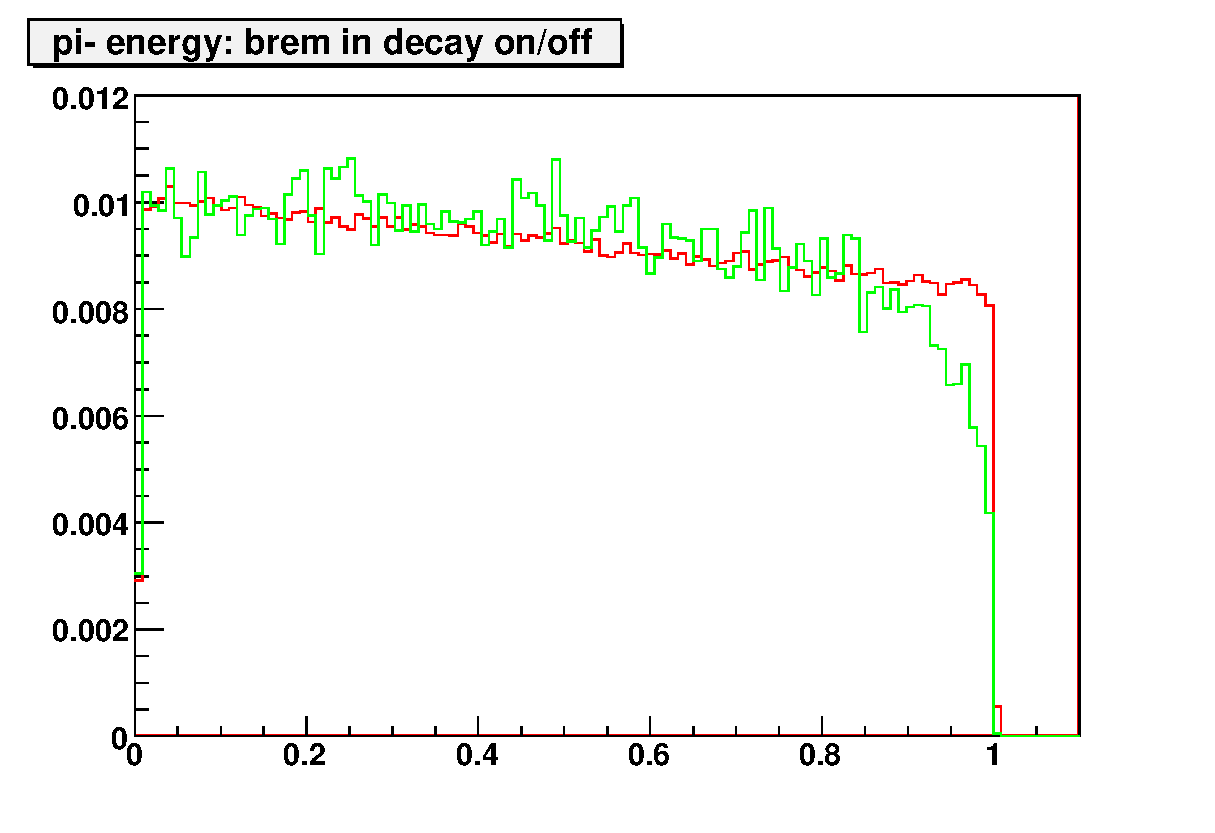
\includegraphics[scale=0.35]{bremdec.eps}
}
\subfigure[bremsshtrahlung from $Z$, $\tau^+ $ and $\tau^- $ decays]{
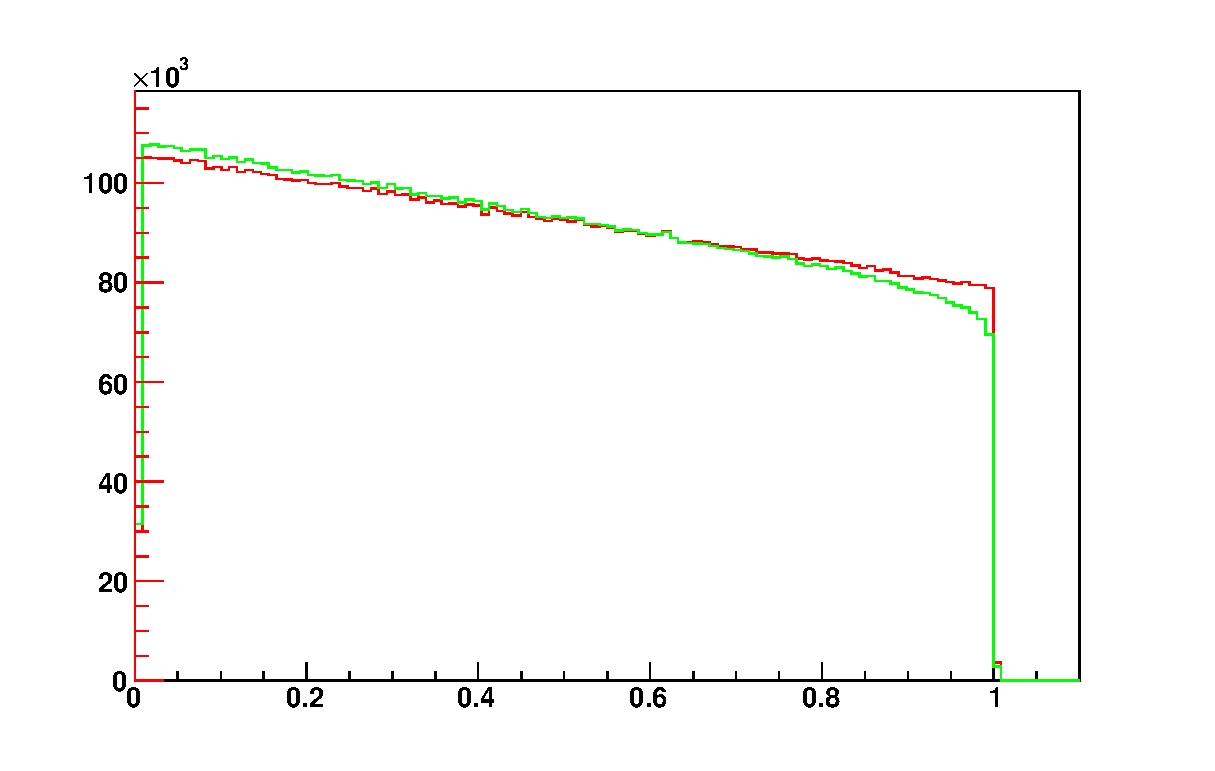
\includegraphics[scale=0.35]{bremall.eps}
}
\caption{ Bremsstrahlung effect for longitudinal spin observable
for cascade decay $Z \to \tau^+ \tau^-$, $\tau^+ \to \pi^+ \nu$,  $\tau^\pm \to \pi^\pm\nu$:
$\pi^+$ energy spectrum in Z rest-frame  is shown. Red line is for 
bremsstrahlung switched off
bremssthahlung off, green, when its effect is included. 
For left hand side plot,  only  bremsstrahlung in  $\tau^+ $ decay is included.
On right hand side bremssthahlung from $Z$ and  $\tau^-$ decays are
 also taken into account.
interface  \label{fig:KKMC}.
}
\end{figure}
\begin{figure}[h!]
\centering
\subfigure[selection C]{
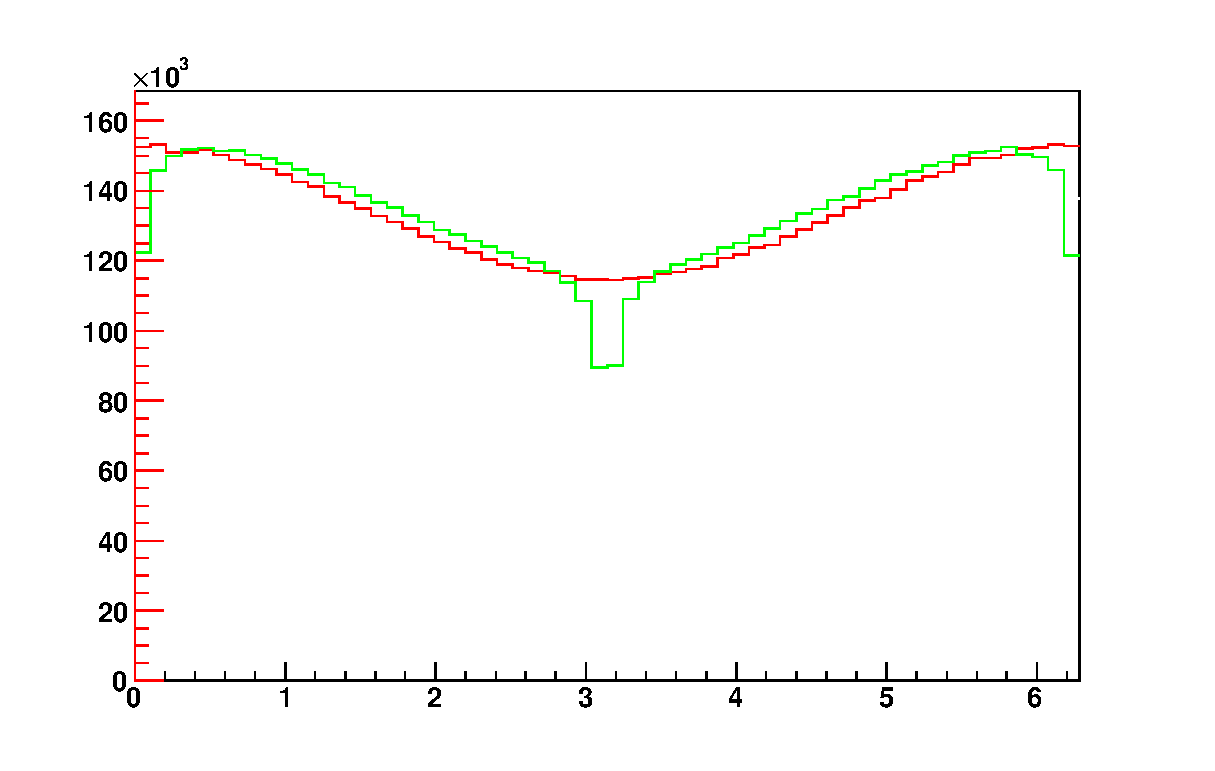
\includegraphics[scale=0.35]{coplanarity-angle-C-photon-over-1-GeV.eps}
}
\subfigure[selection D]{
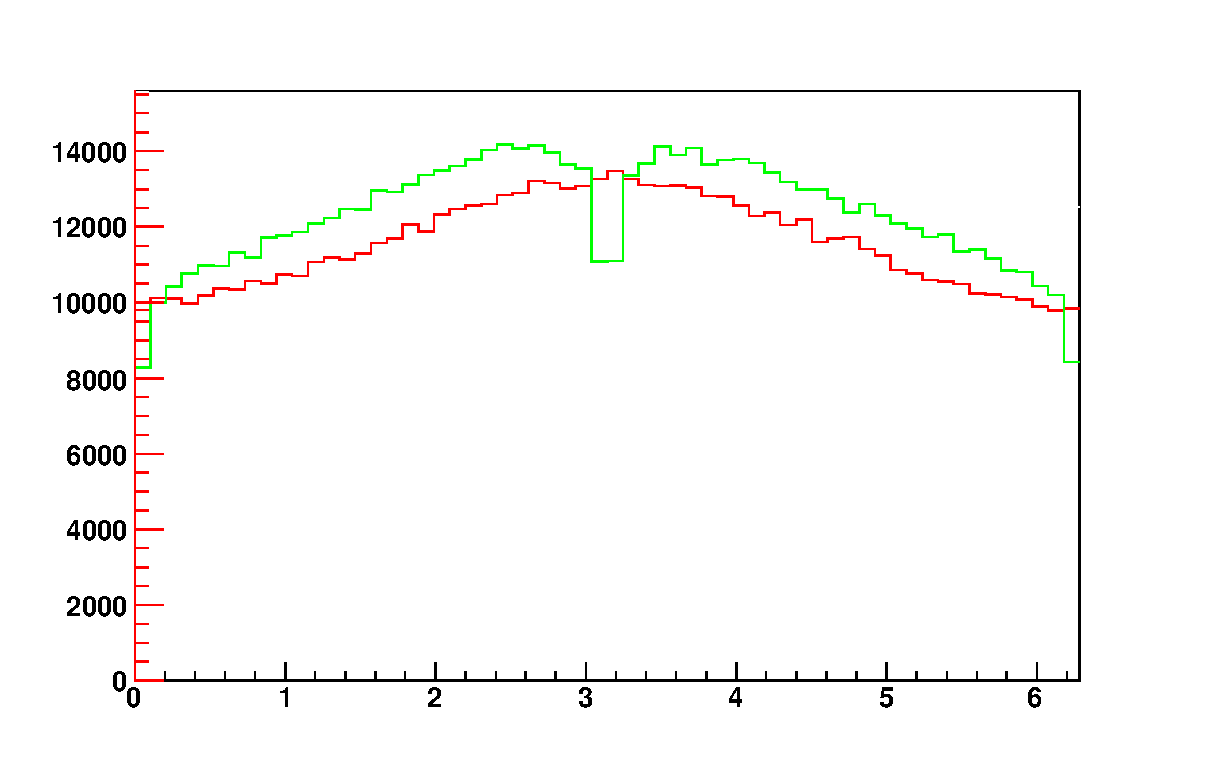
\includegraphics[scale=0.35]{coplanarity-angle-D-photon-over-1-GeV.eps}
}
\caption{Bremsstrahlung effects for transverse spin observable:
In this plot acoplanarity distribution between $\pi^+\rho^+$ and 
$\pi^-\rho^-$ planes in the rest frame of the $\rho+ \rho^-$ pair
for the decay
chain  $H\to \tau^+\tau^-$, $\tau^\pm \to \rho^\pm \nu_\tau$, 
$\rho^\pm \to \pi^\pm \pi^0$, when PHOTOS is generating bremsstrahlung is given.
The plots for scalar higgs are given
Red line is for no bremsstrahlung for the green one,
only events where photons of energy larger than 1 GeV in $H$ rest frame are taken.
Note by comparison with fig from ref~\cite{tauolaC++} that kinematical effect
of hard photons are limited to depletion/increase of content of bins for acoplanarity angle close to $0$, $\pi$ and $2\pi$. For definition of selections C and D see.~\cite{Bower:2002zx}. \label{fig:acoplanarity}
}
\end{figure}
Finally for the sake of debugging we have introduced 'put' methods for the 
control printouts of internal printouts of FORTRAN part of the code.
Then routine PHLUPA \cite{Barberio:1994qi} is activated and one can verify  
for the event offending for example  energy momentum conservation how it is 
constructed. That is quite convenient for tracing inconsistencies in information passed to PHOTOS for example.

\subsection{Algorithm Performance}
Speed testing? Is this even necessary? But maybe someone should check for
memory leaks since I haven't done this.

\newpage

\bibliography{Photos_interface_design}{}
\bibliographystyle{plain}

\newpage

\section*{Task List}
In this section we provide a check-list of incomplete tasks.
This could be used as a guide for project planning and is foreseen
to be a working document. 

(prioritized: {\bf 1} - Highest priority. The program should not be
released without this task being completed. {\bf 2} - Medium priority.
It should be clearly documented for developers and users that this task has not
been completed. {\bf 3} - Lowest priority such as a long term goal 
for the project).

\subsection*{Functionality}
\begin{itemize}
  \item[\ding{111}]{\bf 1} - Example task 1
\end{itemize}

\subsection*{Testing}
\begin{itemize}
  \item[\ding{111}]{\bf 2} - Example task 2
\end{itemize}

\subsection*{Usability}
\begin{itemize}
  \item[\ding{111}]{\bf 1} - Doxygen documentation updated
  \item[\ding{111}]{\bf 3} - etc...
\end{itemize}


\end{document}
